% !TEX root = 00_arbeit.tex

%---------------------------------------------------------------------------------
%% Theorie

\section{Was sind neuronale Netze?}
%\farbig{[Erklärung der neuronalen Netze... vielfältige Anwendungsgebiete... Hier erforderlich Netze zur Zeitreihenvorhersage]}

\begin{wrapfigure}{r}{0.5\textwidth}
    \centering
        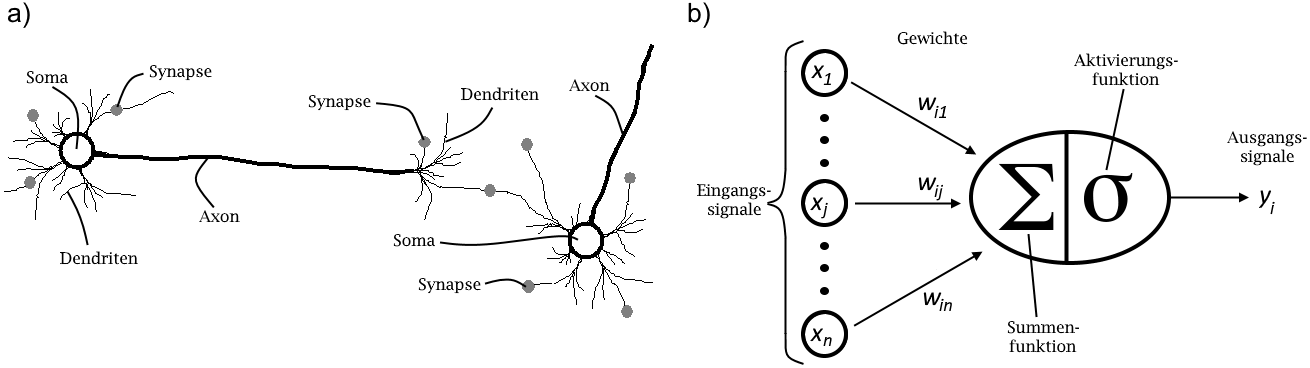
\includegraphics[width=0.5\textwidth]{Bilder/BNN_ANN.png}
    \caption{Gegenüberstellung eines Ausschnittes aus einem biologischen neuronalen Netz a)\protect\footnotemark{} und einem künstlichen neuronalen Netz b).}
    \label{fig:BNN_ANN}
\end{wrapfigure}

\addtocounter{footnote}{-1}%  -1 mal die Gesamtanzahl an Fußnoten in der wrapfigure
\addtocounter{Hfootnote}{-1}% -1 times total number of footnote(mark)s in the wrapfigure
\wrapfigfoot\footnotetext{\autoref{fig:BNN_ANN} a) und \autoref{tab:BNN_ANN} wurden aus\citet[2]{sen_an} übersetzt und angepasst.}
%\citet[\pno~2~ff.]{sen_an}

Künstliche neuronale Netze (engl. artificial neural networks)~(NN) sind augenblicklich eine Disziplin der Computional Intelligence~(CI). Diese fasst verschiedene an die Natur angepasste Berechnungsmethoden zusammen. Weitere Methoden der CI sind Fuzzy-Systeme~(FS), Evolutionäre Algorithmen~(EA), Schwarmintelligenz~(SI) und Künstliche Immunsysteme~(AIS).\fcite[11 ff]{Kroll16} Obwohl sich diese Arbeit wesentlich mit NN beschäftigt wird, wird an dieser Stelle auf weitere CI-Methoden hingewiesen, da in der Literatur hybride CI-Systeme bekannt sind und auch genutzt werden.

Es gibt Problemstellungen die mit klassischen mathematischen Modellen und Algorithmen gar nicht oder nur schwer zu lösen sind. Einige Beispiele wären die Gesichtserkennung oder die Erkennung von menschlicher Sprache. Unser Gehirn erkennt Gesichter und Sprachen aber anscheinend ohne größere Anstrengung.

%\begingroup
\setlength{\intextsep}{0pt}%
%\setlength{\columnsep}{10pt}%
\begin{wraptable}{l}{6.4cm}
    \caption {Analogie zwischen biologischen und künstlichen Neuronen.}
    \begin{tabular}{>{\centering\arraybackslash}m{2.2cm}>{\centering\arraybackslash}m{3.4cm}}
    \hline
    Biologisches\newline Neuron & Künstliches\newline Neuron            \\ \hline \hline
    Soma                & Summen- und\newline Aktivierungsfunktion      \\ 
    Dendrit             & Eingang                                       \\ 
    Axon                & Ausgang                                       \\ 
    Synapse             & Gewicht                                       \\ \hline
    \end{tabular}
    \label{tab:BNN_ANN}
\end{wraptable}
%\endgroup

Aus der Untersuchung von biologischen Abläufen im Nervensystem von Wirbeltieren, wo Sinneseindrücke des Körpers aufgenommen und mit Hilfe diverser neuronaler Netze verarbeitet werden, entstanden Anfang der 40er Jahre des letzten Jahrhunderts\fcite[A1.1:1]{Fiesler96} mathematische Konstrukte die heute als künstliche neuronale Netze bezeichnet werden. 
\autoref{fig:BNN_ANN} zeigt eine Gegenüberstellung von künstlicher und biologischer neuronaler Netze und \autoref{tab:BNN_ANN} die Analogie der Bestandteile eines Neurons. Das zurzeit prominenteste künstliche Neuron (die kleinste Einheit im Netzwerk), dargestellt in \hbox{\autoref{fig:BNN_ANN} b)}, wird nach \citet{perceptron} als Perzeptron bezeichnet. Es summiert zunächst die gewichteten Eingänge:

\begin{equation}
\varphi (x)=\sum_{i=1}^{n}x_{i}\omega_{i}~,
\end{equation}

anschließend wird die gewichtete Summe~$\varphi(x)$ über die Aktivierungsfunktion~$\sigma(x)$ als Ausgang~$y$ an das nächste Neuron übergeben. Klassische Aktivierungsfunktionen sind die \hbox{Heaviside-,} die lineare Schwellwert-, die Fermifunktion und der Tangens Hyperbolicus\footnote{Vgl. \citet[5]{neuralnet_intro} und \citet[39 f]{dkriesel07}.}.\\
Im allgemeinen können NN anhand der folgenden drei Kriterien charakterisiert werden\fcite[7 ff]{characterisation_4}:%

\begin{enumerate}
\item%
Nach der Art des verwendeten Neurons.\\
Dazu gibt es in der Literatur vielfältige Beispiele. \citet{Fiesler96} zählen einige Beispiele im Kapitel B1 auf und weisen auf Unterschiede hin. Als Beispiel wird dort das bereits erwähnte Perceptron beschrieben. Dann gehen sie auf das Neuron des Hopfield-Netzwerkes ein, bei dem das Neuron ein Teilchen beschreibt welches sich in einem Magnetfeld ausrichtet. Ein eher exotischer Vertreter der dort nicht erwähnt wird ist das Fuzzy-Neuron von \citet{fuzzy-neuron}, welches nach der Aktivierung mehrere mögliche Zustände einnehmen kann und seine Anwendung in der Mustererkennug findet.

\item%
Nach der Verbindungsarchitektur.\\
Sie beschreibt wie die Neuronen in einem Netzwerk verbunden sind.
Es werden folgende Architekturen unterschieden:
\begin{itemize}
\item[\textbf{$\bullet$}]%
Autoassoziative: Hierbei fungieren die Eingangs- gleichzeitig als Ausgangsneurone (z.B. das Hopfield-Netzwerk). 

\item[\textbf{$\bullet$}]%
Heteroassoziative: Unterschiedliche Neurone übernehmen die Rolle der Eingangs- bzw. Ausgangsneurone. Hierzu zählen die Multylayer-Perzeptrons (MLP) bei dem mehrere Schichten von mehrzahligen Perzeptronen ein Netzwerk Bilden\fcite[86 ff]{dkriesel07}. Aber auch das Kohonen Netzwerk auch bekannt als Self Organizing Maps (SOM) bei dem die Neuronen sich selbständig anordnen und der Zustand des Netzes als Ausgabe dient\fcite[153 ff]{dkriesel07}.

Zusätzlich wird unterschieden wie die Verbindungen unter den einzelnen Neuronen realisiert sind. Hier wird zwischen zwei Arten unterschieden:

\item[$\circ$]%
Feedforward: Diese Netzwerke bestehen meistens aus Schichten und eine Schicht ist nur mit der jeweils nächsten Schicht verbunden.

\item[$\circ$]%
Recurrent (Feedback): In der deutschsprachigen Literatur als rückgekoppelte oder rekurrente Netze bezeichnet beeinflussen sich diese Netzwerke selbst. Die Neuronen dieser Netzwerke besitzen eine Verbindung entweder zu sich selbst (direkte Rückkoppelung), zu den Neuronen der vorhergehenden Schicht (indirekte Rückkopplung), zu den Neuronen der gleichen Schicht (laterale Rückkopplung) oder vollständig verbundene Netze (Verbindungen zwischen allen Neuronen ausgenommen der direkten Rückkopplung). Durch die Rückkopplung besitzen diese Netzwerke ein "Gedächtnis"~da der vorherige Zustand in die Auswertung der aktuellen Eingangsinformation mit einfließt.\fcite[42 ff]{dkriesel07} Ein Beispiel für ein vollständig verbundenes Netzwerk ist das Hopfield-Netzwerk.

\end{itemize}

\item%
Nach dem Lernalgorithmus. Dieser ermöglicht es das Netzwerk zu trainieren. Die heutzutage benutzten Algorithmen werden in drei Gruppen unterteilt\footnote{Vgl. \citet[55]{dkriesel07}.\label{kriesel55}}:

\begin{itemize}
\item[\textbf{$\bullet$}]%
Supervised learning (überwachtes Lernen): Die Trainingsbeispiele bestehen aus einer Menge an Eingangsinformationen und den dazugehörigen Ausbangsinformationen. Das Ziel ist es die Differenz zwischen der tatsächlichen Ausgabe des Netzwerks und den vorliegenden Ausgangsinformationen zu minimieren.

\item[\textbf{$\bullet$}]%
Reinforcement learning (bestärkendes Lernen): Plakativ kann diese Lernmethode als Zuckerbrot und Peitsche bezeichnet werden bzw. lernen durch Belohnung und Bestrafung. Hierbei werden die Eingangsinformationen zur Verfügung gestellt und die Ausgabe des Netzwerkes wird anhand einer Nutzenfunktion bewertet. Wird die Ausgabe als gut/schlecht angesehen so werden die zugehörigen Verbindungen gestärkt/geschwächt\footnote{Vgl. \citet[201]{dkriesel07} und \citet[A2.3:5]{Fiesler96}.}. 

\item[\textbf{$\bullet$}]%
Unsupervised learning (unüberwachtes Lernen): Wird auch als selbstorganisiertes (self organized) Lernen bezeichnet. Die Trainingsbeispiele bestehen hierbei nur aus Eingansinformationen. Das Netzwerk versucht aus den Eingansinformationen selbstständig Ähnlichkeiten zu erkennen.
Unüberwachte Lernmethoden werden noch unterteilt in konkurrierendes (competitive) und nicht konkurrierendes (noncompetitive) Lernverfahren. Der unterschied besteht darin dass bei dem konkurrierenden Verfahren in einem Netzwerk einzelne Gruppen von Neuronen um die Aktivität konkurrieren\fcite[B3.3:5]{Fiesler96}.

Zusätzlich unterscheidet man unter allen drei Lernmethoden zwei Lernarten\fcite[A2.3:3]{Fiesler96}: 
\item[$\circ$]%
off-line learning: Auch Batch-Trainingsverfahren genannt. Hierbei wird die Netzwerkausgabe nach einer Menge von Eingangsinformationnen ausgewertet und anschließend werden die Gewichte angepasst.

\item[$\circ$]%
on-line learning: Hier werden die Gewichte nach jeder einzelnen Beobachtung der gesamten Eingangsinformationen angepasst. 

\end{itemize}

\end{enumerate}

\citet{characterisation_4} nennen vier Charakterisierungskriterien wobei als viertes Kriterium der Informationsgewinnungsalgorithmus (recall algorithm) aufgeführt ist. In dieser Arbeit wird auf dieses Kriterium verzichtet, da weder \citet{characterisation_4} Beispiele aufführen noch in anderer Literatur dieses Kriterium eine Erwähnung findet.

%\lipsum

%\begin{figure}[h]
%	\centering
%	    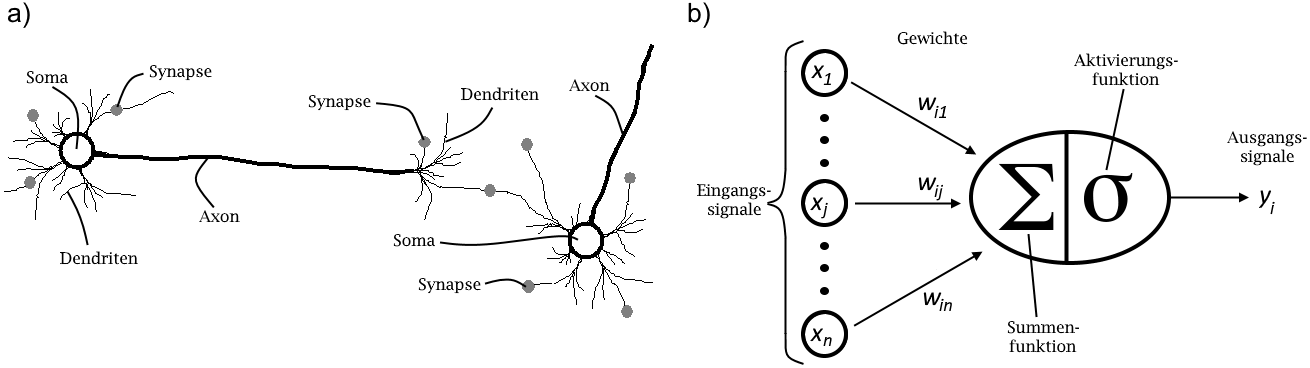
\includegraphics[width=0.5\linewidth]{Bilder/BNN_ANN.png}
%	\caption{Gegenüberstellung eines Ausschnittes aus einem biologischen neuronalen Netz a) und einem künstlichen neuronalen Netz b).}
%	\label{fig:BNN_ANN}
%\end{figure}



%\subsection{Multilayerperzeptrons (MLP)}

%\subsection{Radiale Basisfunktionen (RBF)}

%\subsection{Gegenüberstellung von MLP- und RBF-Netzen}